\documentclass[11pt]{beamer}
\usetheme{Madrid}
\usefonttheme{serif}

\usepackage[utf8]{inputenc}
\usepackage[vietnamese]{babel}
\usepackage[T5]{fontenc}

\usepackage{amsmath}
\usepackage{amsfonts}
\usepackage{amssymb}
\usepackage{graphicx}
\usepackage{booktabs}

\DeclareMathOperator{\sen}{sen}
\DeclareMathOperator{\tg}{tg}

\setbeamertemplate{caption}[numbered]

\author[University of Information Technology]{
    Thành viên thực hiện: \\ 
    Hà Thanh Phong \- 24520024 \\ 
    Hà Xuân Thiện \- 24520031 \\ 
    Trần Quang Trường \- 24521901
}
\title[MiniRAG]{MiniRAG\@: Towards Extremely Simple Retrieval- Augmented Generation}
\newcommand{\email}{email}
\setbeamertemplate{navigation symbols}{} 
\institute[]{University of Information Technology \- VNUHCM} 
\date{\today} 
\bibliographystyle{apalike}

\usepackage{tikz}
\usetikzlibrary{positioning,arrows.meta,calc}
\usepackage{amsmath}

\tikzset{
    img/.style={draw=black, line width=1pt, inner sep=0pt},
    state/.style={circle, draw=black, line width=1.4pt, minimum size=12mm, text=black, font=\Large},
    darr/.style={draw=black, line width=1.4pt, -{Latex[length=4mm,width=3mm]}},
    dlink/.style={draw=black, line width=1.2pt, dashed},
    txt/.style={text=black, font=\Large}
}
\usepackage{graphicx}
\usepackage{animate}
\usepackage{tikz}
\usetikzlibrary{calc}


\usepackage{amsmath}
\usetikzlibrary{arrows.meta,positioning}

\begin{document}

\begin{frame}
    \titlepage\
\end{frame}

\begin{frame}{Mục lục}
    \tableofcontents\
\end{frame}

\section{Bối cảnh bài toán}

\begin{frame}{1. Bối cảnh bài toán}
\textbf{Retrieval-Augmented Generation (RAG)} là một hướng tiếp cận kết hợp giữa
\textbf{truy xuất thông tin} từ kho tri thức bên ngoài và \textbf{sinh ngôn ngữ tự nhiên}
của mô hình ngôn ngữ.

\vspace{0.2cm}
\pause

Nhu cầu triển khai các hệ thống RAG có \textbf{hiệu quả tính toán cao} và
\textbf{chi phí tài nguyên thấp} ngày càng trở nên cấp thiết, đặc biệt trong
các môi trường triển khai bị giới hạn về phần cứng.

\vspace{0.2cm}

Tuy nhiên, khi các kiến trúc RAG hiện có được áp dụng cho
\textbf{Small Language Models (SLMs)}, hiệu năng có thể suy giảm nghiêm trọng
hoặc thậm chí thất bại hoàn toàn do các hạn chế cố hữu của SLMs trong việc
hiểu ngữ nghĩa sâu và diễn giải nhiều bước.
  
\end{frame}

\section{MiniRAG}

\begin{frame}{2. MiniRAG}
    Nhằm khắc phục các thách thức nêu trên, bài báo đề xuất \textbf{MiniRAG},
    một hệ thống RAG được thiết kế theo định hướng đơn giản hóa kiến trúc và
    tối ưu hiệu quả tính toán.

    \vspace{0.2cm}

    MiniRAG giới thiệu hai thành phần kỹ thuật chính:
    \begin{itemize}
        \item \textbf{Heterogeneous Graph Indexing}
        \item \textbf{Lightweight Graph-Based Knowledge Retrieval}
    \end{itemize}
    \vspace{0.5cm}
    Link bài báo: \url{https://arxiv.org/abs/2501.06713}
\end{frame}

\begin{frame}{2. MiniRAG}
    \begin{figure}
        \centering
        
\includegraphics[width=1\textwidth]{fig/1.png}
        \caption{MiniRAG Workflow}
    \end{figure}
\end{frame}

\subsection{Heterogeneous Graph Indexing}

\begin{frame}{2.1 Heterogeneous Graph Indexing}
    \textbf{Ý tưởng chính:} biểu diễn kho tri thức dưới dạng một
    \textbf{đồ thị dị thể} thay vì chỉ lưu trữ các đoạn văn bản độc lập.

    \vspace{0.25cm}

    \begin{itemize}
        \item \textbf{Text chunks:} các đoạn văn bản được phân tách từ tài liệu gốc.
        \item \textbf{Named entities:} các thực thể định danh quan trọng được trích xuất từ văn bản.
        \item \textbf{Edges:} các liên kết biểu diễn quan hệ giữa chunks, entities và các thành phần liên quan.
    \end{itemize}
\end{frame}
\begin{frame}{2.1 Heterogeneous Graph Indexing}
    \begin{figure}
        \centering
        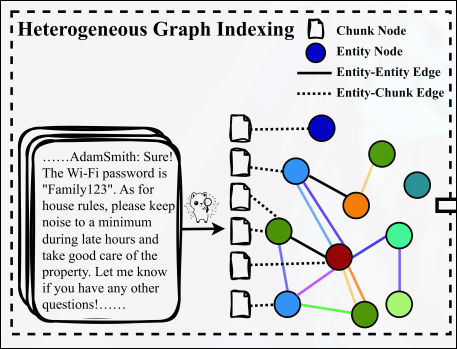
\includegraphics[width=0.7\textwidth]{fig/HGI.png}
        \caption{Heterogeneous Graph Indexing}
    \end{figure}
\end{frame}

\begin{frame}{2.1 Heterogeneous Graph Indexing}
    Quá trình lập chỉ mục trong MiniRAG được hình thức hóa bằng một đồ thị dị thể:

    \vspace{0.25cm}

    \begin{equation}
        D = \mathcal{G} = \left(\{\mathcal{V}_c, \mathcal{V}_e\}, \{\mathcal{E}_{\alpha}, (e_{\beta}, d_{e_{\beta}}) \in \mathcal{E}_{\beta}\}\right)
    \end{equation}

    \vspace{0.2cm}

    \begin{itemize}
        \item $\mathcal{V}_c$: tập các nút biểu diễn \textbf{text chunks}.
        \item $\mathcal{V}_e$: tập các nút biểu diễn \textbf{named entities}.
        \item $\mathcal{E}_{\alpha}$: các cạnh giữa thực thể với thực thể.
        \item $(e_{\beta}, d_{e_{\beta}})$: cạnh giữa thực thể và chunk, kèm mô tả ngữ nghĩa của cạnh.
    \end{itemize}

\end{frame}

\subsection{Lightweight Graph-Based Knowledge Retrieval}
\begin{frame}{2.2 Lightweight Graph-Based Knowledge Retrieval}
    \begin{figure}
        \centering
        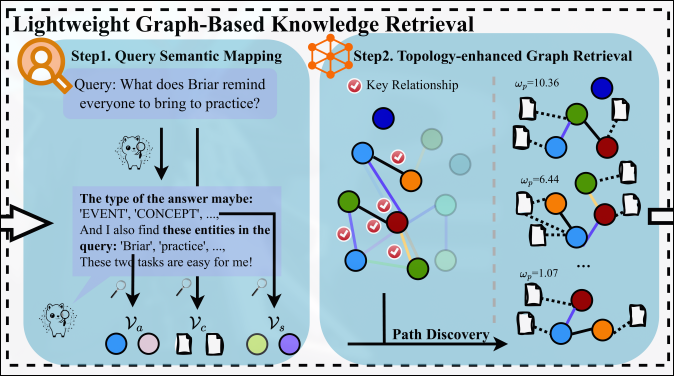
\includegraphics[width=1\textwidth]{fig/LGBKR.png}
        \caption{Lightweight Graph-Based Knowledge Retrieval}
    \end{figure}
\end{frame}

\begin{frame}{2.2.1 Query Semantic Mapping}
    \textbf{Mục tiêu:} ánh xạ truy vấn tự nhiên $q$ vào đồ thị dị thể $\mathcal{G}$ để xác định
    các thực thể và đoạn văn bản có liên quan.

    \vspace{0.2cm}

    \begin{itemize}
        \item Trích xuất tập thực thể truy vấn $\mathcal{V}_q$ từ câu hỏi đầu vào $q$.
        \item So khớp $\mathcal{V}_q$ với các entity nodes $\mathcal{V}_e$ trong đồ thị $\mathcal{G}$.
        \item Xác định các nút khởi đầu $\hat{\mathcal{V}}_s$ và các nút ứng viên câu trả lời $\hat{\mathcal{V}}_a$
        cho bước truy xuất theo topology.
    \end{itemize}
\end{frame}

\begin{frame}{2.2.2 Topology-Enhanced Graph Retrieval}

    \vspace{0.2cm}

    \begin{itemize}
        \item \textbf{Key Relationship Identification:} xác định các cạnh quan trọng
        giữa nút khởi đầu $\hat{\mathcal{V}}_s$ và nút ứng viên câu trả lời $\hat{\mathcal{V}}_a$.

        \begin{equation}
            \omega_e(e) =
            \sum_{\hat{v}_s \in \hat{\mathcal{V}}_s} count(\hat{v}_s, \hat{\mathcal{G}}_{e,k})
            +
            \sum_{\hat{v}_a \in \hat{\mathcal{V}}_a} count(\hat{v}_a, \hat{\mathcal{G}}_{e,k})
        \end{equation}

        \item \textbf{Query-Guided Path Discovery:} xây dựng các đường suy luận liên quan
        đến truy vấn dựa trên cả độ tương đồng ngữ nghĩa và cấu trúc graph.
        \begin{equation}
            \omega_p(p \mid v_q) =
            \omega_v(\hat{v}_s \mid v_q)
            \left(1 +
            \sum_{v \in (p \cap \hat{\mathcal{V}}_a)} count(v,p)
            +
            \sum_{e \in (p \cap \hat{\mathcal{E}}_{\alpha})} \omega_e(e)
            \right)
        \end{equation}
    \end{itemize}

    \begin{itemize}
        \item $\omega_e(e)$: điểm quan trọng của cạnh trong lân cận $k$-hop.
        \item $\omega_p(p \mid v_q)$: điểm của đường suy luận ứng với thực thể truy vấn $v_q$.
    \end{itemize}
\end{frame}

\section{Kết quả thực nghiệm}
    \begin{frame}{3. Kết quả thực nghiệm}
    \begin{figure}
        \centering
        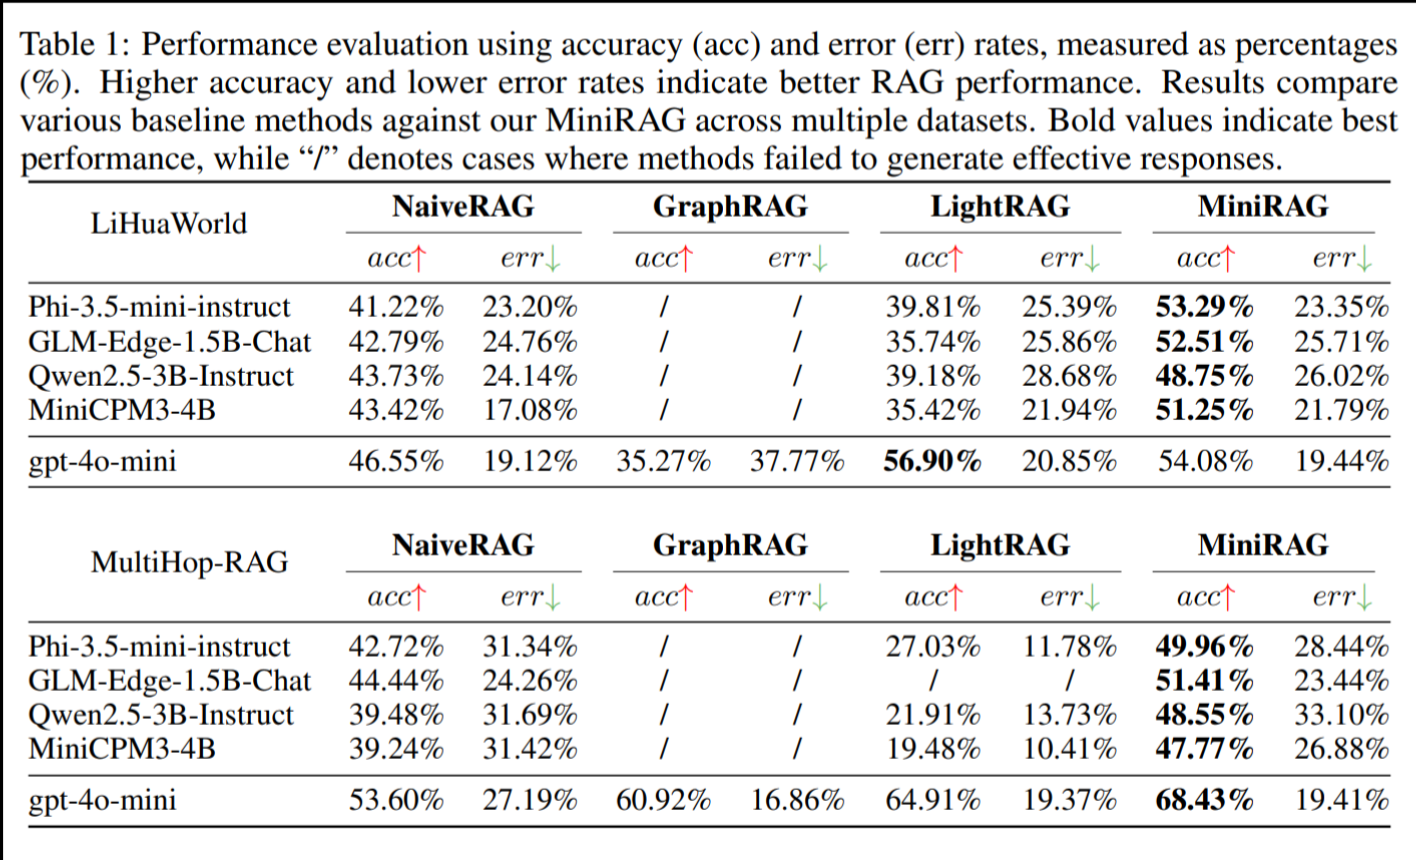
\includegraphics[width=1\linewidth]{fig/exp.png}
        \label{fig:placeholder}
    \end{figure}
    \end{frame}

    \begin{frame}{3. Kết quả thực nghiệm}
        \textbf{OpenBookQA} là tập dữ liệu hỏi đáp trắc nghiệm khoa học, thường dùng để đánh giá khả năng kết hợp giữa fact ngắn và suy luận commonsense.

        \vspace{0.25cm}

        \begin{itemize}
            \item Mỗi câu hỏi có 4 lựa chọn đáp án, trong đó các phương án sai thường chứa từ khóa gây nhiễu.
            \item Các fact trong OpenBookQA thường ngắn và rời rạc, nên không phải lúc nào cũng tạo thành chuỗi suy luận rõ ràng.
            \item Với MiniRAG, đây là một thiết lập khó vì graph của OpenBookQA thưa hơn MultiHop-RAG và dễ bị distractor kéo lệch hướng truy xuất.
            \item Do đó, OpenBookQA phù hợp để kiểm tra khả năng lọc nhiễu, nối bằng chứng và grounding của hệ thống RAG.
        \end{itemize}
    \end{frame}

    \begin{frame}{3. Kết quả thực nghiệm}
        \begin{itemize}
            \item Đánh giá hiệu năng của \textbf{NaiveRAG} và \textbf{MiniRAG} trên các tập dữ liệu \textbf{MultiHop-RAG} và \textbf{tập dữ liệu mới OpenBookQA}.
            \item Sử dụng mô hình \textbf{GLM-Edge-1.5B-Chat}.
        \end{itemize}
    \end{frame}

    \begin{frame}{3. Kết quả thực nghiệm}
    \begin{table}[t]
    \centering
    \small
    \setlength{\tabcolsep}{12pt}
    \renewcommand{\arraystretch}{1.15}

    \begin{tabular}{lcccc}
    \toprule
    \textbf{Dataset}
    & \multicolumn{2}{c}{NaiveRAG}
    & \multicolumn{2}{c}{MiniRAG} \\

    \cmidrule(lr){2-3}
    \cmidrule(lr){4-5}

    & $acc \uparrow$ & $err \downarrow$
    & $acc \uparrow$ & $err \downarrow$ \\

    \midrule
    MultiHop-RAG
    & 60.99\% & 37.64\%
    & 63.41\% & 32.44\% \\

    OpenBookQA
    & 67.60\% & 32.40\%
    & 57.80\% & 42.20\% \\

    \bottomrule
    \end{tabular}
    \caption{Đánh giá so sánh khi sử dụng mô hình GLM-Edge-1.5B-Chat.}
    \end{table}
\end{frame}

    \begin{frame}{3. Kết quả thực nghiệm}
        \begin{itemize}
            \item Đánh giá hiệu năng của \textbf{MiniRAG} trên các tập dữ liệu \textbf{MultiHop-RAG} và \textbf{tập dữ liệu mới OpenBookQA}.
            \item Sử dụng mô hình \textbf{gemma-4-26b-a4b-it}.
        \end{itemize}
    \end{frame}

    \begin{frame}{3. Kết quả thực nghiệm}
    \begin{table}[t]
    \centering
    \small
    \setlength{\tabcolsep}{18pt}
    \renewcommand{\arraystretch}{1.15}

    \begin{tabular}{lcc}
    \toprule
    \textbf{Dataset}
    & \multicolumn{2}{c}{MiniRAG} \\

    \cmidrule(lr){2-3}

    & $acc \uparrow$ & $err \downarrow$ \\

    \midrule
    MultiHop-RAG
    & 83.10\%  & 14.75\% \\


    OpenBookQA
    & 91.40\% & 8.60\% \\

    \bottomrule
    \end{tabular}
    \caption{Đánh giá MiniRAG khi sử dụng mô hình gemma-4-26b-a4b-it.}
    \end{table}
\end{frame}

\section{Phân tích ưu nhược điểm}

\begin{frame}{4. Phân tích}
\begin{block}{Question}
    Endangered pandas are sometimes \\
(A) accidentally dropped into volcanoes \\
(B) confined to enclosures to be viewed by the public \\
(C) found eating corn in the middle of North America \\
(D) made into delicious rare steaks
\end{block}

\begin{itemize}
\item Gold answer label: `B`
\item Gold answer text: `confined to enclosures to be viewed by the public`
\item Original MiniRAG prediction: `A`
\item Fresh rerun prediction: `C`
\end{itemize}
\end{frame}

\section{Phân tích}

\begin{frame}{4. Phân tích}
MiniRAG có lợi khi:
\begin{itemize}
    \item graph giàu liên kết
    \item entity mapping chính xác
    \item câu hỏi cần suy luận nhiều bước
    \item mô hình sinh đủ mạnh để lọc và nối bằng chứng
\end{itemize}

MiniRAG bất lợi khi:
\begin{itemize}
    \item fact ngắn và rời rạc
    \item graph thưa
    \item distractor có từ khóa mạnh
    \item đáp án đúng cần commonsense bridge không có sẵn trong graph
\end{itemize}

\end{frame}


\end{document}
